\section{lg\-Tag\-Arg Class Reference}
\label{classlgTagArg}\index{lgTagArg@{lgTagArg}}
generic tag argument without value  


{\tt \#include $<$lgtagarg.h$>$}

Inheritance diagram for lg\-Tag\-Arg::\begin{figure}[H]
\begin{center}
\leavevmode
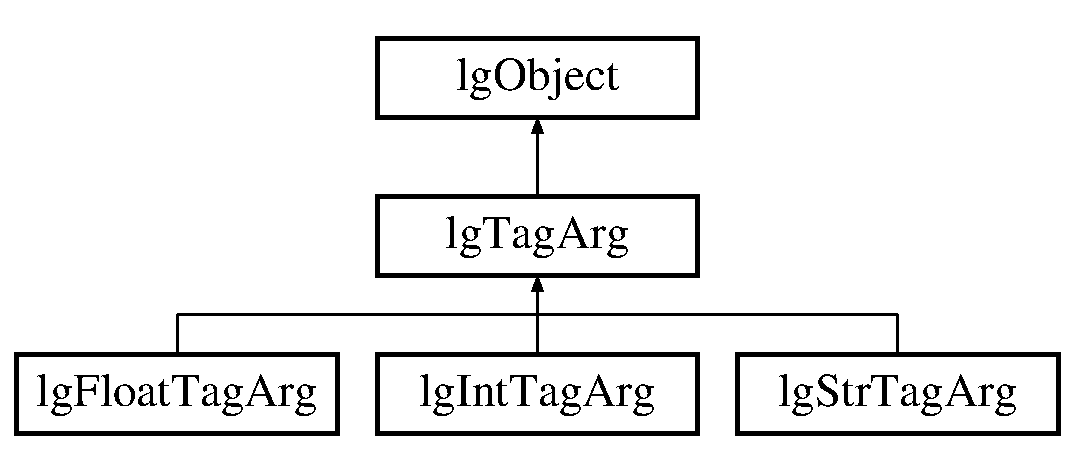
\includegraphics[height=3cm]{classlgTagArg}
\end{center}
\end{figure}
\subsection*{Public Member Functions}
\begin{CompactItemize}
\item 
virtual string {\bf to\-String} ({\bf lg\-Voice} $\ast$seq=NULL)
\item 
{\bf lg\-Tag\-Arg} (const char $\ast$na, const char $\ast$un)
\item 
virtual {\bf $\sim$lg\-Tag\-Arg} (void)
\item 
virtual string {\bf val\-Str} (void)
\item 
virtual int {\bf val\-Int} (void)
\item 
virtual double {\bf val\-Float} (void)
\item 
virtual string {\bf unit} (void)
\item 
const string {\bf name} (void)
\begin{CompactList}\small\item\em argument name, might be \char`\"{}\char`\"{} if unnamed \item\end{CompactList}\end{CompactItemize}
\subsection*{Protected Attributes}
\begin{CompactItemize}
\item 
string {\bf unit\-I}
\begin{CompactList}\small\item\em unit string, is \char`\"{}\char`\"{} for string\-Tag\-Args \item\end{CompactList}\end{CompactItemize}
\subsection*{Private Attributes}
\begin{CompactItemize}
\item 
string {\bf name\-I}
\end{CompactItemize}


\subsection{Detailed Description}
generic tag argument without value 



\subsection{Constructor \& Destructor Documentation}
\index{lgTagArg@{lg\-Tag\-Arg}!lgTagArg@{lgTagArg}}
\index{lgTagArg@{lgTagArg}!lgTagArg@{lg\-Tag\-Arg}}
\subsubsection{\setlength{\rightskip}{0pt plus 5cm}lg\-Tag\-Arg::lg\-Tag\-Arg (const char $\ast$ {\em na}, const char $\ast$ {\em un})}\label{classlgTagArg_a1}


\begin{Desc}
\item[Parameters: ]\par
\begin{description}
\item[{\em 
na}]argument name \item[{\em 
unit}]argument unit \end{description}
\end{Desc}
\index{lgTagArg@{lg\-Tag\-Arg}!~lgTagArg@{$\sim$lgTagArg}}
\index{~lgTagArg@{$\sim$lgTagArg}!lgTagArg@{lg\-Tag\-Arg}}
\subsubsection{\setlength{\rightskip}{0pt plus 5cm}lg\-Tag\-Arg::$\sim${\bf lg\-Tag\-Arg} (void)\hspace{0.3cm}{\tt  [virtual]}}\label{classlgTagArg_a2}




\subsection{Member Function Documentation}
\index{lgTagArg@{lg\-Tag\-Arg}!name@{name}}
\index{name@{name}!lgTagArg@{lg\-Tag\-Arg}}
\subsubsection{\setlength{\rightskip}{0pt plus 5cm}const string lg\-Tag\-Arg::name (void)\hspace{0.3cm}{\tt  [inline]}}\label{classlgTagArg_a7}


argument name, might be \char`\"{}\char`\"{} if unnamed 

\index{lgTagArg@{lg\-Tag\-Arg}!toString@{toString}}
\index{toString@{toString}!lgTagArg@{lg\-Tag\-Arg}}
\subsubsection{\setlength{\rightskip}{0pt plus 5cm}string lg\-Tag\-Arg::to\-String ({\bf lg\-Voice} $\ast$ {\em seq} = NULL)\hspace{0.3cm}{\tt  [virtual]}}\label{classlgTagArg_a0}


get GUIDO string should be redefined in all derived classes 

Reimplemented from {\bf lg\-Object} {\rm (p.\,\pageref{classlgObject_a3})}.

Reimplemented in {\bf lg\-Str\-Tag\-Arg} {\rm (p.\,\pageref{classlgStrTagArg_a0})}, {\bf lg\-Int\-Tag\-Arg} {\rm (p.\,\pageref{classlgIntTagArg_a0})}, and {\bf lg\-Float\-Tag\-Arg} {\rm (p.\,\pageref{classlgFloatTagArg_a0})}.\index{lgTagArg@{lg\-Tag\-Arg}!unit@{unit}}
\index{unit@{unit}!lgTagArg@{lg\-Tag\-Arg}}
\subsubsection{\setlength{\rightskip}{0pt plus 5cm}virtual string lg\-Tag\-Arg::unit (void)\hspace{0.3cm}{\tt  [inline, virtual]}}\label{classlgTagArg_a6}


\index{lgTagArg@{lg\-Tag\-Arg}!valFloat@{valFloat}}
\index{valFloat@{valFloat}!lgTagArg@{lg\-Tag\-Arg}}
\subsubsection{\setlength{\rightskip}{0pt plus 5cm}virtual double lg\-Tag\-Arg::val\-Float (void)\hspace{0.3cm}{\tt  [inline, virtual]}}\label{classlgTagArg_a5}




Reimplemented in {\bf lg\-Str\-Tag\-Arg} {\rm (p.\,\pageref{classlgStrTagArg_a5})}, {\bf lg\-Int\-Tag\-Arg} {\rm (p.\,\pageref{classlgIntTagArg_a3})}, and {\bf lg\-Float\-Tag\-Arg} {\rm (p.\,\pageref{classlgFloatTagArg_a2})}.\index{lgTagArg@{lg\-Tag\-Arg}!valInt@{valInt}}
\index{valInt@{valInt}!lgTagArg@{lg\-Tag\-Arg}}
\subsubsection{\setlength{\rightskip}{0pt plus 5cm}virtual int lg\-Tag\-Arg::val\-Int (void)\hspace{0.3cm}{\tt  [inline, virtual]}}\label{classlgTagArg_a4}




Reimplemented in {\bf lg\-Str\-Tag\-Arg} {\rm (p.\,\pageref{classlgStrTagArg_a4})}, {\bf lg\-Int\-Tag\-Arg} {\rm (p.\,\pageref{classlgIntTagArg_a2})}, and {\bf lg\-Float\-Tag\-Arg} {\rm (p.\,\pageref{classlgFloatTagArg_a4})}.\index{lgTagArg@{lg\-Tag\-Arg}!valStr@{valStr}}
\index{valStr@{valStr}!lgTagArg@{lg\-Tag\-Arg}}
\subsubsection{\setlength{\rightskip}{0pt plus 5cm}virtual string lg\-Tag\-Arg::val\-Str (void)\hspace{0.3cm}{\tt  [inline, virtual]}}\label{classlgTagArg_a3}




Reimplemented in {\bf lg\-Str\-Tag\-Arg} {\rm (p.\,\pageref{classlgStrTagArg_a3})}, {\bf lg\-Int\-Tag\-Arg} {\rm (p.\,\pageref{classlgIntTagArg_a4})}, and {\bf lg\-Float\-Tag\-Arg} {\rm (p.\,\pageref{classlgFloatTagArg_a3})}.

\subsection{Member Data Documentation}
\index{lgTagArg@{lg\-Tag\-Arg}!nameI@{nameI}}
\index{nameI@{nameI}!lgTagArg@{lg\-Tag\-Arg}}
\subsubsection{\setlength{\rightskip}{0pt plus 5cm}string {\bf lg\-Tag\-Arg::name\-I}\hspace{0.3cm}{\tt  [private]}}\label{classlgTagArg_r0}


\index{lgTagArg@{lg\-Tag\-Arg}!unitI@{unitI}}
\index{unitI@{unitI}!lgTagArg@{lg\-Tag\-Arg}}
\subsubsection{\setlength{\rightskip}{0pt plus 5cm}string {\bf lg\-Tag\-Arg::unit\-I}\hspace{0.3cm}{\tt  [protected]}}\label{classlgTagArg_p0}


unit string, is \char`\"{}\char`\"{} for string\-Tag\-Args 



The documentation for this class was generated from the following files:\begin{CompactItemize}
\item 
{\bf lgtagarg.h}\item 
{\bf lgtagarg.cpp}\end{CompactItemize}
